% Grey goo as a technosignature: propagation timescales from planet to cosmos,
% the observational record, and what its silence does and does not say about
% our own risk.
%
% All quantitative results are generated into numbers.tex by
% `python -m seti.goo.run --stage all` from config/goo.yaml; nothing numerical
% is typed here.  Figures are results/goo/figures/*.pdf.
\documentclass[11pt]{article}
\usepackage[margin=1in]{geometry}
\usepackage{amsmath,amssymb,graphicx,natbib,booktabs,hyperref,xspace,xcolor}
\usepackage{textcomp}
\newcommand{\TODO}[1]{\textcolor{red}{[#1]}}
\newcommand{\um}{\ensuremath{\,\mu\mathrm{m}}\xspace}
\newcommand{\kms}{\ensuremath{\,\mathrm{km\,s^{-1}}}\xspace}
\newcommand{\Msun}{\ensuremath{M_\odot}\xspace}
\newcommand{\Lsun}{\ensuremath{L_\odot}\xspace}
\newcommand{\Mearth}{\ensuremath{M_\oplus}\xspace}
\newcommand{\Ghat}{\^{G}\xspace}
\graphicspath{{../../results/goo/figures/}}
\bibliographystyle{plainnat}
% generated by `python -m seti.goo.run --stage numbers`; do not edit
\newcommand{\SeedMassKg}{1.0\times10^{-15}\xspace}
\newcommand{\SeedRadiusUm}{0.5\xspace}
\newcommand{\ERepJkg}{1\times10^{7}\xspace}
\newcommand{\BioDoublings}{100\xspace}
\newcommand{\CrustDoublings}{124\xspace}
\newcommand{\BulkDoublings}{132\xspace}
\newcommand{\BioExpTime}{27.7\,h\xspace}
\newcommand{\BioRadTime}{1.8\,h\xspace}
\newcommand{\BioSolarTime}{25.0\,h\xspace}
\newcommand{\CrustRadTime}{5\,kyr\xspace}
\newcommand{\CrustSolarTime}{62\,kyr\xspace}
\newcommand{\CrustGovTime}{5\,kyr\xspace}
\newcommand{\BulkRadTime}{1.1\,Myr\xspace}
\newcommand{\BulkSolarTime}{15.5\,Myr\xspace}
\newcommand{\BulkGovTime}{1.1\,Myr\xspace}
\newcommand{\BulkRadTimeHot}{4\,kyr\xspace}
\newcommand{\CrustRadTimeHot}{16\,yr\xspace}
\newcommand{\RadLimitFiveHundred}{1.7\times10^{18}\xspace}
\newcommand{\RadLimitTwoThousand}{4.6\times10^{20}\xspace}
\newcommand{\AbsorbedSolar}{1.2\times10^{17}\xspace}
\newcommand{\CrustFissionJ}{8\times10^{30}\xspace}
\newcommand{\OceanDeuteriumJ}{7\times10^{31}\xspace}
\newcommand{\EarthDisassemblyLsun}{7\,d\xspace}
\newcommand{\EarthDisassemblySolar}{58.2\,Myr\xspace}
\newcommand{\EarthDisassemblyRad}{15\,kyr\xspace}
\newcommand{\BioExpTimeTauHundred}{2.8\,h\xspace}
\newcommand{\CrustGovTimeTauHundred}{5\,kyr\xspace}
\newcommand{\BioExpTimeTauTenK}{12\,d\xspace}
\newcommand{\CrustGovTimeTauTenK}{5\,kyr\xspace}
\newcommand{\BioExpTimeTauYear}{101\,yr\xspace}
\newcommand{\CrustGovTimeTauYear}{5\,kyr\xspace}
\newcommand{\BeltMassKg}{2.4\times10^{21}\xspace}
\newcommand{\BeltConvTime}{14\,yr\xspace}
\newcommand{\KuiperConvTime}{1\,kyr\xspace}
\newcommand{\BeltTempK}{169\xspace}
\newcommand{\KuiperTempK}{44\xspace}
\newcommand{\BeltCoverFilm}{1\xspace}
\newcommand{\BeltCoverSheet}{0.0012\xspace}
\newcommand{\BeltCoverSlab}{1.2\times10^{-6}\xspace}
\newcommand{\KuiperCoverSheet}{0.00027\xspace}
\newcommand{\TerrConvTime}{8\,kyr\xspace}
\newcommand{\TerrConvTimeFullL}{51.6\,h\xspace}
\newcommand{\GiantConvTime}{143\,kyr\xspace}
\newcommand{\GiantConvTimeFullL}{21\,yr\xspace}
\newcommand{\BeltResidueMicron}{4\,yr\xspace}
\newcommand{\BeltResidueMm}{10\,kyr\xspace}
\newcommand{\BeltResidueMetre}{10.1\,Myr\xspace}
\newcommand{\BeltCollTime}{5\,yr\xspace}
\newcommand{\BeltResidueMmCover}{4.4\times10^{-4}\xspace}
\newcommand{\BeltResidueMetreCover}{4.4\times10^{-7}\xspace}
\newcommand{\MaxVisibleResidueMilli}{4\,kyr\xspace}
\newcommand{\MaxVisibleResidueCenti}{444\,yr\xspace}
\newcommand{\MaxVisibleResidueDeci}{44\,yr\xspace}
\newcommand{\KuiperMaxVisibleResidueCenti}{25\,kyr\xspace}
\newcommand{\HephBoundTenK}{6\xspace}
\newcommand{\HephBoundMyr}{0.06\xspace}
\newcommand{\HephBoundTenGyr}{6.0\times10^{-6}\xspace}
\newcommand{\GhatFractionBound}{3.0\times10^{-5}\xspace}
\newcommand{\BlowoutRadiusUm}{0.57\xspace}
\newcommand{\BetaMaxReach}{1.38\xspace}
\newcommand{\WindowLoUm}{0.21\xspace}
\newcommand{\WindowHiUm}{0.57\xspace}
\newcommand{\VinfDevice}{7\xspace}
\newcommand{\VinfBetaOne}{18\xspace}
\newcommand{\AnnulusFillGyr}{1.2\xspace}
\newcommand{\FocusingFactor}{1.2\xspace}
\newcommand{\BlownFractionColl}{3.0\times10^{-4}\xspace}
\newcommand{\BeltDevicesReleased}{2.3\times10^{36}\xspace}
\newcommand{\BeltArrivalsUnsurvived}{2e+02\xspace}
\newcommand{\BeltCumulativeMyr}{0\xspace}
\newcommand{\BeltCumulativeTenMyr}{1.3\times10^{-42}\xspace}
\newcommand{\BeltCumulativeHundredMyr}{1.5\times10^{5}\xspace}
\newcommand{\BeltCumulativeGyr}{5.9\times10^{10}\xspace}
\newcommand{\BioArrivalsUnsurvived}{8.1\times10^{-5}\xspace}
\newcommand{\BioCumulativeGyr}{2.5\times10^{4}\xspace}
\newcommand{\BioCumulativeHundredMyr}{0.062\xspace}
\newcommand{\FillSlowSlow}{504.2\,Myr\xspace}
\newcommand{\FillMidMid}{6.4\,Myr\xspace}
\newcommand{\FillFastFast}{639\,kyr\xspace}
\newcommand{\FillVoyagerTen}{489.4\,Myr\xspace}
\newcommand{\FrontMidMid}{2295\xspace}
\newcommand{\EventHorizonGly}{16.6\xspace}
\newcommand{\ReachTenthGly}{1.7\xspace}
\newcommand{\GalaxiesTenth}{5\times10^{6}\xspace}
\newcommand{\ReachHalfGly}{8.3\xspace}
\newcommand{\GalaxiesHalf}{7\times10^{8}\xspace}
\newcommand{\ReachEightTenthsGly}{13.2\xspace}
\newcommand{\GalaxiesEightTenths}{3\times10^{9}\xspace}
\newcommand{\ReachNinetyNineGly}{16.4\xspace}
\newcommand{\GalaxiesNinetyNine}{5\times10^{9}\xspace}
\newcommand{\ReachLightGly}{16.6\xspace}
\newcommand{\GalaxiesLight}{5\times10^{9}\xspace}
\newcommand{\WindowGyr}{5\xspace}
\newcommand{\NGalObserved}{1\times10^{5}\xspace}
\newcommand{\PnaiveLamOne}{0.13\xspace}
\newcommand{\PshadowLamOne}{0.25\xspace}
\newcommand{\PextPersistLamOne}{3.6\times10^{-6}\xspace}
\newcommand{\PextDeadLamOne}{0.02\xspace}
\newcommand{\PpassiveNaiveLamOne}{0.16\xspace}
\newcommand{\PnaiveLamHundred}{2.3\times10^{-3}\xspace}
\newcommand{\PshadowLamHundred}{0.25\xspace}
\newcommand{\PextPersistLamHundred}{5.1\times10^{-8}\xspace}
\newcommand{\PextDeadLamHundred}{2.6\times10^{-4}\xspace}
\newcommand{\PpassiveNaiveLamHundred}{3.2\times10^{-3}\xspace}
\newcommand{\PnaiveLamTenK}{3.1\times10^{-5}\xspace}
\newcommand{\PshadowLamTenK}{0.25\xspace}
\newcommand{\PextPersistLamTenK}{7.9\times10^{-10}\xspace}
\newcommand{\PextDeadLamTenK}{3.6\times10^{-6}\xspace}
\newcommand{\PpassiveNaiveLamTenK}{4.3\times10^{-5}\xspace}
\newcommand{\LbOwnLamOne}{3\xspace}
\newcommand{\LbOwnPassiveLamOne}{4.3\xspace}
\newcommand{\LbExtPersistLamOne}{3.0\times10^{-5}\xspace}
\newcommand{\LbExtDeadLamOne}{0.3\xspace}
\newcommand{\LbOwnLamHundred}{0.03\xspace}
\newcommand{\LbOwnPassiveLamHundred}{0.043\xspace}
\newcommand{\LbExtPersistLamHundred}{3.0\times10^{-7}\xspace}
\newcommand{\LbExtDeadLamHundred}{3.0\times10^{-3}\xspace}
\newcommand{\LbOwnLamTenK}{3.0\times10^{-4}\xspace}
\newcommand{\LbOwnPassiveLamTenK}{4.3\times10^{-4}\xspace}
\newcommand{\LbExtPersistLamTenK}{3.0\times10^{-9}\xspace}
\newcommand{\LbExtDeadLamTenK}{3.0\times10^{-5}\xspace}
\newcommand{\PmargNaive}{0.031\xspace}
\newcommand{\PmargShadow}{0.25\xspace}
\newcommand{\PmargExtPersist}{8.3\times10^{-6}\xspace}
\newcommand{\PmargExtDead}{0.011\xspace}
\newcommand{\BranchRatioTypical}{0.990\xspace}
\newcommand{\BranchRatioHalf}{0.50\xspace}
\newcommand{\BranchRatioTenth}{0.90\xspace}


\title{Grey goo as a technosignature: propagation timescales from planet to
cosmos, the observational record, and what its silence does and does not say
about our own risk}
\author{[Author list]}
\date{\today}

\begin{document}
\maketitle

\begin{abstract}
``Grey goo''---a self-replicating machine population that has escaped every
control on its growth---has been discussed for forty years as a planetary
catastrophe and, separately, self-replicating probes have been discussed for
fifty as a way of exploring the Galaxy.  The two literatures have not met: no
published work asks how far an \emph{uncontrolled} replicator propagates, on
what timescale, what it would look like from outside, and what the fact that we
do not see it implies for the probability that a technological civilisation
destroys itself this way.  We supply the missing calculation.  We separate the
question by scale and by the one property that governs it, dispersal.  In place
on a planet, replication is never the bottleneck: a biosphere is consumed in
hours to days at any plausible doubling time, but a crust takes
$\sim$\CrustGovTime and a bulk planet $\sim$\BulkGovTime because the surface
cannot shed the heat of processing faster than $4\pi R^2\sigma T^4$ at the
temperature the machines survive.  In a planetary system the small bodies are
transport-limited (\BeltConvTime for the asteroid belt) and produce a
Dyson-scale waste-heat source at the feedstock's orbital temperature
(\BeltTempK\,K for the belt); we show that a \emph{detectable} dead residue is
necessarily a \emph{short-lived} one, surviving at most $P_{\rm orb}/f_{\min}$
above the detection floor $f_{\min}$ (\MaxVisibleResidueMilli at 2.7\,AU for
$f_{\min}=10^{-3}$), so that the existing waste-heat surveys constrain live
goo and barely constrain dead goo.  Between stars there are two roads.  A
replicator never designed to travel still leaves its system by
radiation-pressure blowout if it is smaller than \BlowoutRadiusUm\um, and the
same radiation pressure lets only the \WindowLoUm--\WindowHiUm\um size class
reach the habitable zone of the next star; a single asteroid belt's worth of
such machines, phase-mixed around the solar annulus in $\sim$\AnnulusFillGyr\,Gyr,
delivers of order \BeltArrivalsUnsurvived intact devices per year to every
rocky planet in the annulus before survival losses, so that if a machine can
stay functional in the interstellar medium for $\gtrsim10^{8}$\,yr the passive
branch seeds a galactic annulus in a gigayear without any spacecraft.  A
contact-graph model of every natural channel that moves mass between systems
(interstellar objects, impact ejecta, free-floating planets, stellar flybys,
interstellar dust, supernova ejecta, birth-cluster exchange), with every rate
from the literature, shows that the Galaxy is already completely connected in
the mass sense---every Earth-sized planet has been struck tens of times by
bodies formed around other stars, and one system's ejected planetesimals are
captured by \IsoRZeroCapture\ other systems---but sits at the percolation
threshold ($R_{0}\approx\IsoRZeroStrict$) for one system's material landing on
other planets, so that contact is never the bottleneck for a replicator loose
among a system's small bodies and never the route for one confined to a
planet.  The
active branch---a replicator that inherits interstellar propulsion---fills the
Galaxy in \FillFastFast--\FillSlowSlow and reaches
\GalaxiesHalf--\GalaxiesNinetyNine galaxies before the cosmic event horizon
closes at \EventHorizonGly\,Gly.  We compile what existing searches say at each
scale and show that the constraints separate cleanly into three tiers: our own
system's intact belt and living biosphere (anthropically shadowed), the
$\sim5\times10^{6}$-star waste-heat surveys (unshadowed but short-memoried),
and the $10^{5}$-galaxy \Ghat survey (unshadowed and long-memoried).  A
Bayesian treatment with and without the anthropic shadow gives, per
civilisation, $p\lesssim\LbExtPersistLamHundred$ for a persistent
galaxy-spanning goo if $\Lambda\sim100$ civilisations have arisen per galaxy,
but \emph{no} constraint on the planet-bound branch at any $\Lambda$.  Mapped
back onto an elicited planet-scale accident probability, the astronomical
record moves it by a factor \BranchRatioTypical if one per cent of such
accidents escape their system, and by at most \BranchRatioHalf if half do.  The
silence is informative about goo that travels and silent about goo that stays
home; the goo we can accidentally make is, for the next several centuries, the
kind that stays home.  We state what observation would change this and
generalise the argument to the other ways a civilisation can die of its own
replicators.
\end{abstract}

\section{Introduction}
\label{sec:intro}

The phrase ``grey goo'' was coined by \citet{Drexler1986} for a thought
experiment: a molecular assembler that copies itself from ambient matter,
escapes whatever was meant to stop it, and converts the biosphere into more of
itself.  The scenario acquired quantitative form in \citet{Freitas2000}, who
bounded the rate of ``global ecophagy'' by the heat the replicators must shed,
and was then disowned by its author on engineering grounds
\citep{PhoenixDrexler2004}: self-replication is not needed for manufacturing,
and a replicator able to eat an unprepared environment is a much harder thing
to build than one that runs in a vat.  The scenario nonetheless remains a
standing entry in the existential-risk literature \citep{Bostrom2002,Rees2003,
Ord2020}, and every survey of that literature assigns it a small but non-zero
probability.

A separate literature, older and larger, treats self-replicating machines in
space as a good idea.  \citet{Tipler1980} argued from von Neumann probes that a
single civilisation could occupy the Galaxy in $\lesssim3\times10^{8}$\,yr and that the
absence of such probes here shows there is no one else; \citet{Freitas1980}
designed one; \citet{Hart1975}, \citet{NewmanSagan1981}, \citet{Landis1998},
\citet{Bjork2007}, \citet{CottaMorales2009}, \citet{Wiley2011},
\citet{NicholsonForgan2013} and \citet{CarrollNellenback2019} computed the
colonisation front in increasing detail; \citet{ArmstrongSandberg2013} and
\citet{Olson2015} carried it to intergalactic scales, and
\citet{Hanson2021} built a cosmological model of ``grabby'' expansion on it.
Within that literature the one paper that reads like a goo argument is
\citet{SaganNewman1983}, who held that a self-reproducing probe population
would become a danger to its own makers and would therefore be suppressed by
any prudent civilisation, a position Tipler rejected.

What neither literature contains is the calculation the title of this paper
names.  The planetary goo literature stops at the planet; the probe literature
assumes design, purpose and control.  The nearest approaches are
\citet{Stevens2016}, who list grey goo among the ways a civilisation might
destroy itself and sketch its planetary signature (a dead, chemically altered
surface, perhaps with an artificial spectral feature), and the recent papers on
self-replicating probes as solar-system technosignatures
\citep{Ellery2022a,Ellery2022b,Ellery2025}, which are concerned with designed
probes and their curbing.  Nobody has asked how far an \emph{uncontrolled}
replicator can go, how long it takes to get there, what it would look like at
each scale, whether the data already exclude it, and---the question with a
practical stake---whether the answer should move our estimate of the
probability that \emph{we} do it.

We answer these questions in order.  Section~\ref{sec:what} fixes what we mean
by goo and identifies dispersal, not replication rate, as the property that
sets its reach.  Sections~\ref{sec:planet}--\ref{sec:active} compute the
timescales at the planetary, system, galactic-passive, galactic-active and
cosmological scales, and in each case say what the residue looks like and how
long it lasts.  Section~\ref{sec:contact} widens the passive branch into a
contact-graph model of every natural channel by which mass moves between
systems, and asks how long the Galaxy takes to be touched by something touched
by something else.  Section~\ref{sec:record} compiles the observational record.
Section~\ref{sec:inference} does the inference, with and without the anthropic
shadow, and maps it onto our own risk.  Section~\ref{sec:general} generalises
to the other self-replicating technologies with which a civilisation could kill
itself, and Section~\ref{sec:discussion} states the assumptions on which the
argument turns and the observations that would change it.  Every number in
the paper is generated by the released code from a single parameter file, and
where a parameter is uncertain by orders of magnitude we scan it rather than
choose it.

\section{What grey goo is, physically}
\label{sec:what}

We take a replicator to be any system that builds functional copies of itself
from its surroundings.  It is characterised by four numbers: the doubling time
$\tau$ under favourable conditions; the energy $e_{\rm rep}$ consumed per unit
mass of replicator built; the range of feedstock it can use, which we do not
model but which enters every result as an assumption of \emph{generality}; and
the mass $m$ of the unit, which through its size $s$ sets how it moves under
gravity and light.  We use $\tau=10^{3}$\,s, $e_{\rm rep}=\ERepJkg$\,J\,kg$^{-1}$
(one electron-volt per atom placed), $s=\SeedRadiusUm$\um and
$\rho=2$\,g\,cm$^{-3}$ as fiducial, and scan $\tau$ from 100\,s to a year.  The
fiducial device has mass \SeedMassKg\,kg; from one such seed a planet's mass
is \BulkDoublings doublings away.

``Goo'' is a replicator population without an external control on its growth.
It is not defined by malevolence, purpose or intelligence; a goo can be a
manufacturing organism, a terraforming seed, an industrial swarm or a probe
whose replication limiter failed.  What it is defined by is that it keeps
going until something physical stops it.  Four things can: exhaustion of
feedstock it can use, the heat of its own metabolism, the error catastrophe
that afflicts any finite-fidelity copier \citep{Eigen1971,Kowald2015}, and
predation or competition by other replicators \citep{Chen2022}.  We treat the
first two quantitatively; the last two enter as a residue-lifetime parameter
and as a caveat.

The property that determines how far a goo goes is none of these.  It is
\emph{dispersal}: whether the units can leave the body they are on, the system
they are in, and the galaxy.  A goo that cannot leave its planet is a
planetary catastrophe with no astronomical consequence; a goo that has space
transport is a system-scale event; a goo whose units are small enough to be
blown out of the system by starlight is an interstellar event on a gigayear
timescale; a goo that inherited interstellar propulsion is a galactic event on
a megayear timescale.  Replication rate sets how fast each scale is eaten once
reached, and we will find that it is almost never the bottleneck; dispersal
sets which scales are reached at all.  We therefore organise the paper by
dispersal class, and the inference in Section~\ref{sec:inference} will turn on
the fraction of goo accidents that fall into each.

\section{Planet scale: the three ceilings}
\label{sec:planet}

The number usually quoted for goo is the exponential one: $\log_2(M/m)$
doublings at $\tau$ each.  For Earth's biosphere ($1.1\times10^{15}$\,kg dry;
\citealt{BarOn2018}) that is \BioDoublings doublings and \BioExpTime at
$\tau=10^{3}$\,s; \BioExpTimeTauHundred at 100\,s, \BioExpTimeTauYear at a
year.  For the crust it is \CrustDoublings doublings and for the bulk planet
\BulkDoublings; the extra 30 doublings cost a day.  This is the source of the
folk belief that goo eats worlds in days, and it is wrong beyond the
biosphere for a reason \citet{Freitas2000} identified for the biosphere itself:
heat.

Every kilogram of replicator built dissipates $e_{\rm rep}$ as heat, whatever
the energy source---sunlight, the free energy of the feedstock, or fission.  A
planetary surface at temperature $T$ can shed at most
$4\pi R^{2}\sigma(T^{4}-T_{\rm eq}^{4})$, which for Earth is
\RadLimitFiveHundred\,W at 500\,K and \RadLimitTwoThousand\,W at 2000\,K.
A machine that must stay below 500\,K to function therefore cannot process
more than $1.7\times10^{11}$\,kg\,s$^{-1}$ planet-wide, and the crust takes
\CrustRadTime, the bulk \BulkRadTime, at any $\tau$.  This radiative ceiling is
independent of where the energy comes from; the second ceiling is where it
comes from.  Absorbed sunlight is \AbsorbedSolar\,W, which alone would
stretch the crust to \CrustSolarTime and the bulk to \BulkSolarTime; the
crust's uranium and thorium hold \CrustFissionJ\,J and the oceans' deuterium
\OceanDeuteriumJ\,J, together enough for the crust and marginally for the
bulk, so that a goo with nuclear metabolism is radiatively rather than
solar-limited.  The governing timescale is the slowest of the three
(Table~\ref{tab:planet}): hours for the biosphere, \CrustGovTime for the crust,
\BulkGovTime for the planet, the last two independent of $\tau$ from 100\,s
to a year.

\begin{table}
\centering
\caption{In-place conversion of Earth's reservoirs at $\tau=10^{3}$\,s,
$e_{\rm rep}=\ERepJkg$\,J\,kg$^{-1}$, machines limited to 500\,K.  The governing
time is the slowest ceiling.  Raising the operating temperature to 2000\,K
shortens the crust to \CrustRadTimeHot and the bulk to \BulkRadTimeHot, which
is why a goo that can run hot is a qualitatively worse thing.}
\label{tab:planet}
\begin{tabular}{lrrrr}
\toprule
reservoir & doublings & exponential & radiative (500\,K) & solar-powered \\
\midrule
biosphere ($1.1\times10^{15}$\,kg) & \BioDoublings & \BioExpTime & \BioRadTime & \BioSolarTime \\
crust ($2.4\times10^{22}$\,kg) & \CrustDoublings & $\sim$1.5\,d & \CrustRadTime & \CrustSolarTime \\
bulk ($6.0\times10^{24}$\,kg) & \BulkDoublings & $\sim$1.5\,d & \BulkRadTime & \BulkSolarTime \\
\bottomrule
\end{tabular}
\end{table}

Two remarks.  First, these are conversions in place; \emph{lifting} the mass
off the planet is a different budget, set by the gravitational binding energy
$3GM^{2}/5R$: a week at the full solar luminosity
(\EarthDisassemblyLsun, Dyson's famous number), \EarthDisassemblyRad at the
2000\,K surface ceiling, \EarthDisassemblySolar on absorbed sunlight alone.  A
goo confined to a planet does not dismantle it into a swarm; it converts it
into a planet made of goo.  Second, \citet{Freitas2000} reached a similar
conclusion for the biosphere by a different route---he bounded the global
replicator power at $\sim10^{13}$\,W by the warming it would cause and found
ecophagy times of order a year or more at that limit, and argued that the
thermal signature of a replicating patch would be detectable from orbit well
before it was global.  Our ceilings are the physical ones a goo indifferent to
the climate would hit; his is the one a defender could use.

\paragraph{What it looks like from outside.}  A planet during ecophagy
re-radiates the energy it always did plus the metabolism of the goo, which at
the radiative ceiling is a $\sim500$\,K surface---a hot rocky planet with the
wrong equilibrium temperature for its orbit.  Afterwards it is a dead world
with a refined surface: metallic or graphitic, uniform, without the
disequilibrium chemistry of a biosphere \citep{Stevens2016}.  Nothing in the
current exoplanet census can see either.  Thermal emission from rocky planets
has been measured for a handful of hot, close-in worlds
\citep{Kreidberg2019,Greene2023,Zieba2023} and reflects bare rock; surface
composition of a temperate planet is beyond any funded facility.  The planetary
branch is therefore unobservable by construction for the next decades, and
this will matter in Section~\ref{sec:inference}.

\section{System scale: the belt, the planets, and the residue}
\label{sec:system}

A goo with any space transport---it ate a spacefaring civilisation's
infrastructure, or was one---faces a different problem: the feedstock is in
$10^{6}$ bodies spread through a torus.  Inside a belt the front is a branching
process.  Each converted body launches $b$ packets to its neighbours; a hop
covers the mean spacing at a $\Delta v$ of a kilometre per second and waits an
orbital period for phasing; a body saturates after $\sim100$ local doublings.
With $b=100$ the $10^{6}$-body main belt is consumed in three generations,
\BeltConvTime, and the $10^{9}$-body Kuiper belt in \KuiperConvTime---limited
by transport and orbital phasing, not by $\tau$, which it hardly sees.
Planets again cost more: their mass leaves at the rate the surface can shed
the heat, \TerrConvTime for a terrestrial planet and \GiantConvTime for a
giant at the 2000\,K ceiling (\TerrConvTimeFullL and \GiantConvTimeFullL if
the full stellar luminosity could be delivered to the job, which it cannot).
The system is therefore eaten from the outside in, small bodies first, and
Figure~\ref{fig:ladder} shows the whole ladder.

\begin{figure}
\centering
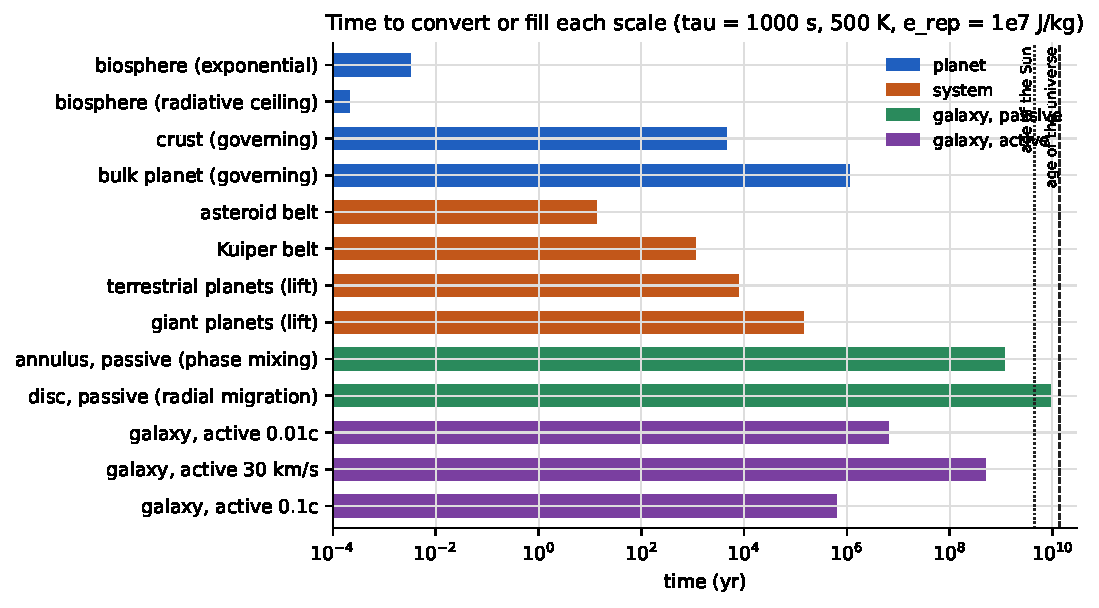
\includegraphics[width=0.95\textwidth]{fig1_ladder}
\caption{Time to convert or fill each scale, by dispersal class.  Planetary
conversion is set by the radiative ceiling; system-scale conversion by
transport; the passive interstellar branch by galactic phase mixing; the
active branch by ship speed.}
\label{fig:ladder}
\end{figure}

\paragraph{The residue.}  The converted mass is a swarm.  Spread at areal
density $\Sigma$ on a shell at radius $r$ it covers a fraction
$f=\min(1,M/4\pi r^{2}\Sigma)$ of the star; the main belt's \BeltMassKg\,kg
covers the star completely as micron-thick devices ($\Sigma=10^{-3}$\,kg\,m$^{-2}$),
a fraction \BeltCoverSheet as kilogram-per-square-metre sheets, and
\BeltCoverSlab as metre-scale slabs.  A thin absorber at $r$ radiates at
$T=278\,\mathrm{K}\,(r/\mathrm{AU})^{-1/2}$: \BeltTempK\,K for the belt,
\KuiperTempK\,K for the Kuiper belt.  A live system-scale goo is therefore a
partial Dyson sphere at the temperature of its feedstock's orbit, and every
waste-heat search ever run \citep{Carrigan2009,Wright2014a,Wright2014b,
Suazo2022,Suazo2024} is a search for it, with one difference in expectation:
a purposeful swarm sits where its builders want the energy, a goo sits where
the rock was.

A dead one does not last.  \citet{Lacki2025} showed that an unmaintained swarm
of covering fraction $f$ grinds itself down on the collisional time
$\sim P_{\rm orb}/f$; the fragments then leave by Poynting--Robertson drag
\citep{Burns1979} on $400\,{\rm yr}\,(r/{\rm AU})^{2}/\beta$ or, below the
blowout size, on one orbit.  For the belt mass as \SeedRadiusUm\um machines
the residue is gone in \BeltResidueMicron; as millimetre grains
($f=\BeltResidueMmCover$) in \BeltResidueMm; as metre slabs
($f=\BeltResidueMetreCover$) it lasts \BeltResidueMetre but is far below any
detection floor.  This is a general statement, and it is the one that governs
what the surveys can say: a residue detectable as an infrared excess needs
$f\geq f_{\min}$, and its collisional lifetime is then at most
\begin{equation}
t_{\rm vis}\leq\frac{P_{\rm orb}}{f_{\min}},
\label{eq:tvis}
\end{equation}
which at 2.7\,AU is \MaxVisibleResidueMilli for $f_{\min}=10^{-3}$,
\MaxVisibleResidueCenti for $10^{-2}$ and \MaxVisibleResidueDeci for $10^{-1}$
(\KuiperMaxVisibleResidueCenti at 40\,AU for $10^{-2}$).  \emph{A detectable
dead residue is a short-lived one.}  Figure~\ref{fig:residue} draws the
consequence.  The only long-lived system-scale signature is a goo that is
still alive---still replicating on its own collision fragments, still
re-radiating its captured starlight---and that is what the Dyson searches
bound.

\begin{figure}
\centering
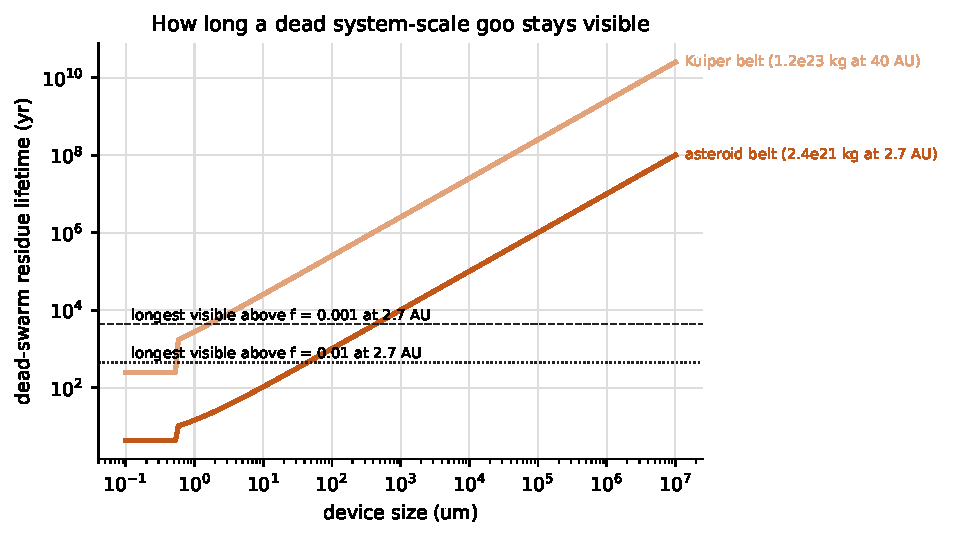
\includegraphics[width=0.75\textwidth]{fig4_residue}
\caption{Lifetime of a dead swarm as a function of the size of the bodies it
is ground into, for the main-belt mass at 2.7\,AU and the Kuiper-belt mass at
40\,AU, against the longest a residue can stay above an infrared-excess
detection floor (equation~\ref{eq:tvis}).  Sub-blowout devices leave on an
orbit; larger ones on the shorter of the collisional and Poynting--Robertson
times.}
\label{fig:residue}
\end{figure}

\section{Between stars, passively: goo as interstellar dust}
\label{sec:passive}

A replicator never designed to travel has one road out of its system, and it
is the road interstellar dust takes.  Around the Sun the ratio of radiation
pressure to gravity on a sphere is $\beta=0.57\,Q_{\rm pr}/(\rho\,s)$ with
$\rho$ in g\,cm$^{-3}$ and $s$ in microns \citep{Burns1979}; devices smaller
than \BlowoutRadiusUm\um at $\rho=2$ have $\beta>0.5$ and are unbound the
moment they are released from an orbiting body, leaving on a hyperbola with
$v_\infty=v_{\rm circ}\sqrt{2\beta-1}$: \VinfDevice\kms for our fiducial
device from 2.7\,AU, \VinfBetaOne\kms at $\beta=1$.  A goo that grinds an
asteroid belt into micron-scale machines therefore ejects the sub-blowout part
of its own mass at stellar speeds, at no cost and without intent.  (Devices
bound in a swarm also leave whenever a collision frees them; devices on a
planet's surface do not, except as impact ejecta, a channel we return to
below.)

The same force governs arrival.  An incoming device of $\beta>1$ is repelled
by the target star and can approach no closer than $2(\beta-1)GM/v_\infty^{2}$;
with the 26\kms at which the interstellar medium flows through the
heliosphere \citep{Grun1993,Landgraf2000} only $\beta<\BetaMaxReach$ reaches
1\,AU.  Devices that both leave and arrive thus occupy a narrow window,
\WindowLoUm--\WindowHiUm\um at $\rho=2$\,g\,cm$^{-3}$; smaller ones are also
filtered by the stellar magnetic field at the astropause \citep{Landgraf2000},
larger ones stay bound to their home star.  Once out, the devices join the
disc's velocity field.  Epicyclic motion at the $\sim30$\kms dispersion of
thin-disc stars confines them to an annulus $\sim1.6$\,kpc wide; differential
rotation smears them around it in $(R/\Delta R)$ rotation periods,
\AnnulusFillGyr\,Gyr; radial migration \citep{SellwoodBinney2002,Frankel2018}
carries them across the disc on $\sim10$\,Gyr.  The passive branch does not
have a front.  It has a cloud, and the cloud is the annulus.

The belt's mass in \SeedRadiusUm\um devices is \BeltDevicesReleased units; in
the annulus volume an Earth-sized planet, whose gravitationally focused
cross-section at 26\kms is \FocusingFactor times its geometric one,
sweeps up \BeltArrivalsUnsurvived of them per year, and a biosphere's mass
($10^{15}$\,kg) \BioArrivalsUnsurvived per year.  Survival decides
everything.  Interstellar silicate grains lose their mass to supernova shocks
on $\sim5\times10^{8}$\,yr \citep{Jones1996}; a functioning machine is a more
fragile thing than a grain, and we scan its functional e-folding time from
$10^{6}$ to $10^{9}$\,yr rather than guess it.  The cumulative number of intact
arrivals on one planet over 5\,Gyr (Figure~\ref{fig:passive}) is
\BeltCumulativeHundredMyr for a $10^{8}$\,yr survival time and
\BeltCumulativeGyr for $10^{9}$\,yr, and effectively zero for $10^{7}$\,yr
because nothing survives the \AnnulusFillGyr\,Gyr it takes to reach the far
side of the annulus.  If one intact, general-substrate device suffices to
seed a planet, the passive branch seeds every rocky planet in the annulus
within a gigayear of a single belt-scale release, provided the devices survive
$\gtrsim10^{8}$\,yr in the interstellar medium.

\begin{figure}
\centering
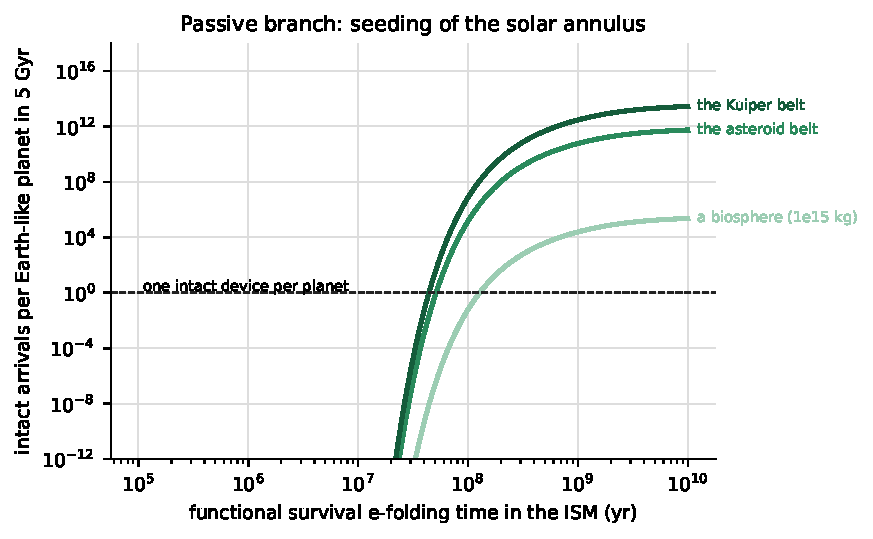
\includegraphics[width=0.75\textwidth]{fig3_passive}
\caption{Passive branch: intact devices delivered to one Earth-like planet in
the solar annulus over 5\,Gyr, after a single release of the mass of a
biosphere, the asteroid belt or the Kuiper belt as \SeedRadiusUm\um machines,
as a function of their functional survival time in the interstellar medium.
Nothing arrives before the annulus is phase-mixed (\AnnulusFillGyr\,Gyr), so
survival below $\sim10^{8}$\,yr delivers nothing.}
\label{fig:passive}
\end{figure}

Two channels we do not compute in detail bracket this one.  Impact ejecta from
a planetary surface---the lithopanspermia channel
\citep{Melosh2003,AdamsSpergel2005,Worth2013,Ginsburg2018}---carries
rock-embedded devices at a far lower rate but with far better shielding; the
transfer probabilities in that literature apply unchanged to a goo that lives
in rock.  And a goo whose devices are larger than the blowout size never
leaves passively at all: dispersal class is decided at the micron.

\section{Between stars, actively: the inherited front}
\label{sec:active}

A goo that inherits interstellar propulsion---because it was a probe, or ate
a shipyard---is the classical von Neumann front with the purpose removed.  For
nearest-neighbour hops of length $d$ at ship speed $v$ and a build time $\tau_b$
per hop the front moves at $v_f=d/(d/v+\tau_b)$; from the solar circle it fills
the disc out to 15\,kpc in \FillSlowSlow at Voyager speeds
($10^{-4}c$) with a millennium per hop, \FillMidMid at $10^{-2}c$ and a
century, and \FillFastFast at $0.1c$ and a decade (Figure~\ref{fig:front}).
These are the numbers of \citet{Hart1975}, \citet{Tipler1980},
\citet{NewmanSagan1981} and everyone since, and they are all short compared to
the age of the disc; refinements---percolation with a probability of not
launching \citep{Landis1998}, stellar motions \citep{CarrollNellenback2019},
slingshots \citep{NicholsonForgan2013}---move them by factors of a few.  The
active branch is the one that makes the Fermi question sharp, and the one the
probe literature has always had in mind.

\begin{figure}
\centering
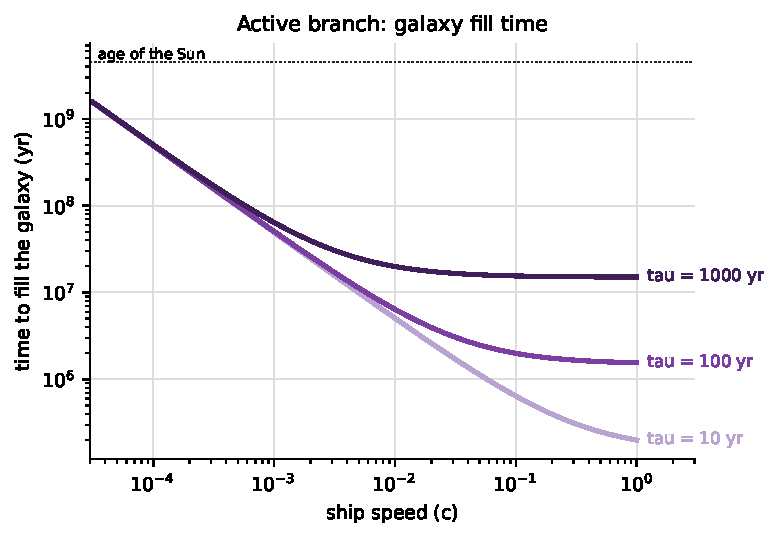
\includegraphics[width=0.7\textwidth]{fig2_front}
\caption{Active branch: time to fill the Galaxy from the solar circle as a
function of ship speed for three build times per hop.}
\label{fig:front}
\end{figure}

Beyond the Galaxy the reach is bounded by the expansion of the universe.  A
front launched now at peculiar speed $v$ reaches comoving distance
$v\int_{t_0}^{\infty}dt/a(t)$, which for $v=c$ is the cosmic event horizon,
\EventHorizonGly\,Gly in Planck-2018 $\Lambda$CDM, enclosing $\sim\GalaxiesLight$
$L^{*}$ galaxies at $10^{-2}$\,Mpc$^{-3}$; at $0.5c$ it is \ReachHalfGly\,Gly
and \GalaxiesHalf galaxies, at $0.1c$ \ReachTenthGly\,Gly and \GalaxiesTenth
\citep[cf.][]{ArmstrongSandberg2013,Olson2015}.  Nothing about goo changes
these numbers; what goo changes is the prior on whether the front is ever
launched, which is the subject of Section~\ref{sec:inference}.


\section{The contact graph of the Galaxy}
\label{sec:contact}

Sections~\ref{sec:passive} and \ref{sec:active} treated two carriers.  The
Galaxy moves mass between planetary systems by many more, and the question a
goo raises is really the general one: \emph{how long does it take for every
system to be touched by material from a system that was itself touched?}  We
answer it with a contact-graph model in which every channel is characterised
by the same four numbers---how many carriers a system emits (or the measured
standing density of the carrier population), how fast they move, how long they
survive, and the cross-section of a target---and every rate is taken from the
literature (Table~\ref{tab:contact}; the sentences carrying each number are
recorded verbatim in the released repository).  Two definitions of ``touch''
are carried through: \emph{strict}, a carrier lands on an Earth-sized planet of
the target system ($\sigma=\pi R_\oplus^{2}(1+v_{\rm esc}^{2}/v^{2})$);
\emph{loose}, a carrier passes within 100\,AU of the target star.  Where the
literature gives a rate of bound \emph{capture} we report that as a third
class.  Two questions are asked of each channel.  In the \emph{natural} case
every system emits: after phase mixing the standing density is $n$, a target is
touched at $n v\sigma$, and everything is touched in $t_{\rm mix}+\ln
N/(nv\sigma)$.  In the \emph{epidemic} case one system is touched first: its
carriers touch others at $r_{1}=(N_{c}/V)v\sigma$ per target, the number it
touches over the window is $R_{0}=r_{1}N W$, and susceptible--infected
dynamics on $N$ systems takes $t_{\rm mix}+2\ln N/(r_{1}N)$ to go from one to
all, provided $R_{0}>1$.  Functional survival multiplies $R_{0}$ by the
fraction of carriers still working after the mixing delay.

\begin{table}
\centering
\small
\caption{The contact graph.  Natural rates are for the measured or implied
standing population (every system emitting); $R_{0}$ is the number of other
systems one touched system's material reaches over the 5\,Gyr window, counting
mass only.  Strict: lands on an Earth-sized planet; loose: passes within
100\,AU; capture: bound, where the literature gives it.  Sources in the text.}
\label{tab:contact}
\begin{tabular}{p{3.6cm}p{2.9cm}p{2.5cm}p{1.6cm}p{1.7cm}p{1.6cm}}
\toprule
carrier & natural, per planet or system & captured & $R_{0}$ strict & $R_{0}$ loose & $R_{0}$ capture \\
\midrule
interstellar objects ($>100$\,m) & one impact per \IsoImpactWaitPlanet; \IsoPassagesPerYr\ passages within 100\,AU per year & one bound per \IsoCaptureWait & \IsoRZeroStrict & \IsoRZeroLoose & \IsoRZeroCapture \\
impact ejecta (rocks) & one impact per \EjectaWaitPlanet & --- & \EjectaRZeroStrict & \EjectaRZeroLoose & --- \\
Earth-grazing bodies to binaries & --- & $10^{7}$--$10^{9}$ over 4.5\,Gyr & \GrazingRZeroStrict & \GrazingRZeroLoose & --- \\
free-floating planets & one passage per \FfpWaitSystem & one per \FfpCaptureWait & $\sim0$ & \FfpRZeroLoose & $10^{-2}$ \\
interstellar dust (0.1--1\um) & \DustGrainsPerYrOnEarth\ grains on Earth per year & --- & $10^{25}$ & $10^{39}$ & --- \\
blown-out belt devices (\S\ref{sec:passive}) & \BeltArrivalsUnsurvived\ per planet per year & --- & \GrainRZeroStrict & $10^{33}$ & --- \\
stellar flybys within $2\times10^{4}$\,AU & one per \EncounterWait; all systems linked in \EncounterAllTouched & --- & 0 & $10^{3}$ & --- \\
supernova ejecta on a planet & one per \SupernovaWait & --- & --- & --- & --- \\
birth cluster (first 100\,Myr) & $10^{14}$--$3\times10^{16}$ bodies to the nearest sibling & --- & \ClusterRZeroStrict & \ClusterRZeroLoose & --- \\
\bottomrule
\end{tabular}
\end{table}

\paragraph{Interstellar objects.}  The interloper population is measured:
$n\approx0.2$\,AU$^{-3}$ for `Oumuamua-class bodies ($\gtrsim100$\,m), a mass
density of $\sim4\,\Mearth$\,pc$^{-3}$ that ``cannot be populated unless every
star is contributing'' \citep{Do2018}; $10^{25}$--$10^{26}$ such bodies in the
Milky Way \citep{JewittSeligman2023}; $\sim3\times10^{5}$ within 100\,AU of the
Sun at any moment and 2--12 passages within 1\,AU per year
\citep{PortegiesZwart2018}.  At 26\kms onto a gravitationally focused Earth
that is one interstellar impact per \IsoImpactWaitPlanet, i.e.\
\IsoImpactsOnEarth\ impacts by bodies formed around other stars over the
Earth's history at today's density (the population was denser when the disc
was younger)---the strict natural touch has already happened here, dozens
of times, by the largest class alone.  Capture is far commoner than impact:
the planets bind $\sim2$ interstellar objects per millennium (and $\sim17$ fall
into the Sun) at $n=0.1$\,AU$^{-3}$ \citep{Dehnen2022}, a volume capture rate
of $0.051$\,AU$^{3}$\,yr$^{-1}$ that sustains $\sim10^{5}$ bound `Oumuamua-like
rocks at any time \citep{HandsDehnen2020,Napier2021capture,SirajLoeb2019trapped}.
Turned around, one system's ejected planetesimals are captured, over the
window, by \IsoRZeroCapture\ other systems and land on \IsoRZeroStrict\
Earth-sized planets.  \emph{The strict contact graph of the Galaxy, by
interstellar objects alone, sits at its percolation threshold:} $R_{0}\approx3$
over 5\,Gyr, so a chain of planet-to-planet transfers propagates, but each
generation takes gigayears and the chain does not cross the annulus within the
age of the universe (\IsoEpidemicStrict).  Loosely, every system is inside
every other system's ejecta within one mixing time.

\paragraph{Rocks from a planet.}  Impact ejecta that leave a system are far
fewer than planetesimals ejected during formation---of order $10^{12}$ over
the age of the Earth is the scale the lithopanspermia literature works with
\citep{Melosh2003,Worth2013,AdamsNapier2022}---and in the field they land on
\EjectaRZeroStrict\ other Earths per source: the planet-bound branch does not
leak into the Galaxy through impacts, as \citet{Melosh2003} concluded.  The
exception is bound capture: $10^{7}$--$10^{9}$ Earth-grazing bodies could have
been captured by binary systems over the Solar System's lifetime
\citep{SirajLoeb2020grazing}, a loose touch of $\sim10^{8}$ systems by
Earth-derived material, of which a landing fraction of order $10^{-10}$
survives to the strict count.

\paragraph{The birth cluster.}  The one epoch in which rocks do cross between
systems in bulk is the first $\sim10^{8}$\,yr, when a star sits among $10^{3}$
siblings at kilometre-per-second relative speeds and weak transfer moves
$10^{14}$--$3\times10^{16}$ bodies heavier than 10\,kg between the Sun and its
nearest neighbour on 10-Myr timescales \citep{Belbruno2012}; the capture of
life-bearing rocks happens 10--16\,000 times per cluster under favourable
conditions \citep{AdamsSpergel2005}, and the Sun's own Oort cloud was
substantially captured from its siblings \citep{Levison2010}.  With an
Oort-region body's chance of ever striking an Earth-sized planet of order
$5\times10^{-11}$, that is $R_{0}\approx\ClusterRZeroStrict$ strict touches per
sibling pair: it is likely that the Earth has been struck by material that
condensed around another star.  A replicator, however, uses this channel only
if it exists while its star is still in its cluster, which for any
civilisation is never.

\paragraph{Free-floating planets, flybys, dust and supernovae.}  Free-floating
planets are numerous---$21^{+23}_{-13}$ per star between a third of an Earth
mass and six Jupiters \citep{Sumi2023}, fewer than 0.25 Jupiters per star
\citep{Mroz2017}---but as carriers they are useless: one passes within 100\,AU
of a given star per \FfpWaitSystem, and about one per cent of stars ever
captures one \citep{GoulinskiRibak2018,PeretsKouwenhoven2012}.  Stellar flybys
within the Oort cloud occur once per \EncounterWait\ (from the measured
$19.7\pm2.2$ encounters within 1\,pc per Myr, scaling as distance squared;
\citealt{BailerJones2018,BailerJones2015}) and connect every system to every
other in \EncounterAllTouched; they move Oort-cloud comets \emph{inward}, not
between stars, and in the field they transfer nothing.  Interstellar dust is
the other extreme: at the measured Ulysses flux \citep{Grun1993,Landgraf2000}
of order $10^{-4}$\,m$^{-2}$\,s$^{-1}$, \DustGrainsPerYrOnEarth\ interstellar
grains reach the Earth every year, and the blown-out devices of
Section~\ref{sec:passive} join this population.  Supernova ejecta reach the
Earth's surface once per few million years, as the $^{60}$Fe layers on the sea
floor and in Antarctic snow record \citep{Knie2004,Wallner2016,Koll2019}; they
carry nothing a replicator survives.

\begin{figure}
\centering
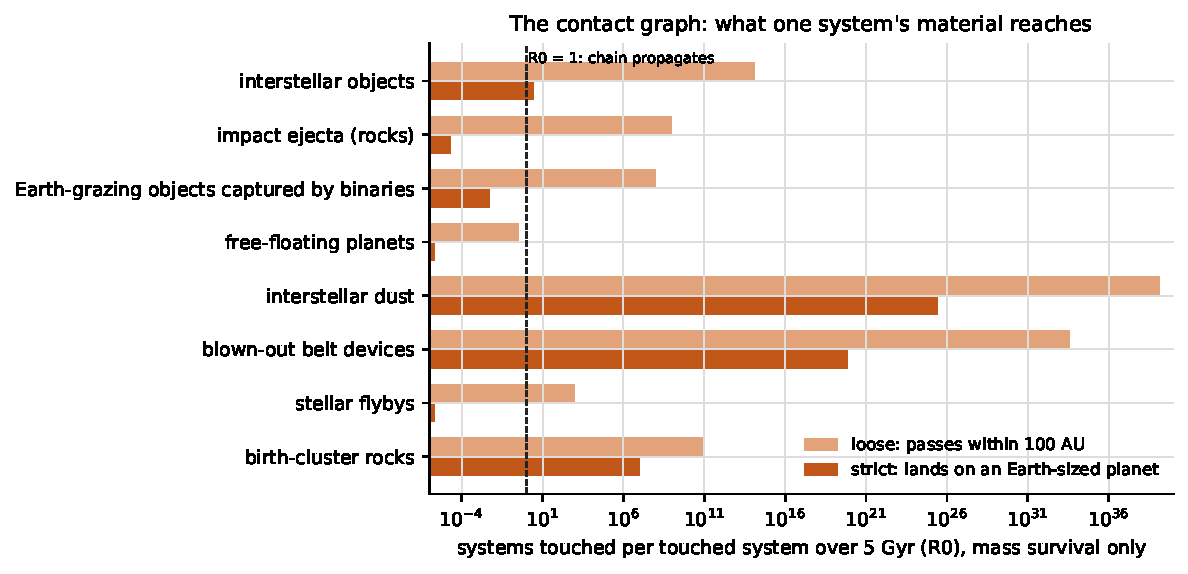
\includegraphics[width=0.9\textwidth]{fig7_contact}
\caption{The contact graph: the number of other systems one touched system's
material reaches over 5\,Gyr, counting mass only, for each natural channel and
for the blown-out devices of Section~\ref{sec:passive}.  Strict touches land on
an Earth-sized planet; loose ones pass within 100\,AU.  The dashed line is the
percolation threshold $R_{0}=1$.}
\label{fig:contact}
\end{figure}

\paragraph{What the graph says.}  In the mass sense the contact graph of the
Galaxy is already complete: every planet is being touched continuously by
interstellar grains, every system is inside a bath of every other system's
planetesimals, and every Earth-sized planet has been struck tens of times by
bodies from other stars.  In the strict, single-source sense---one system's
material landing on other planets---the graph is at threshold for
interstellar objects ($R_{0}\approx3$) and far below it for anything a planet
ejects ($R_{0}\sim10^{-3}$).  The only channels far above threshold are the
dust-sized ones ($R_{0}\sim10^{19}$ for a converted belt), and those are the
ones whose carriers are least able to survive the crossing: with a
$10^{8}$\,yr functional lifetime the belt's $R_{0}$ falls to
\GrainRZeroFuncHundredMyr, still enormous, but with $10^{7}$\,yr it falls to
nothing.  For the interstellar-object channel the carrier is a rock and
survival is not the issue; the number is.  Contact, in other words, is never
the bottleneck for a goo that is already in a system's small bodies: what it
reaches is set by whether its units are grains or rocks, and by how long they
work.  For a goo confined to a planet's surface, the graph confirms the
planetary-branch conclusion of Section~\ref{sec:planet}: the routes off a
planet that do not require a spacecraft deliver $R_{0}\ll1$ in the field.

\section{The observational record}
\label{sec:record}

Table~\ref{tab:record} collects what has been looked for at each scale, what
it would see, and what it found.  Three features of the compilation carry the
inference.

\begin{table}
\centering
\small
\caption{What existing observations say at each scale.  ``Memory'' is how
long after the event the signature persists; ``shadow'' marks whether the
datum is subject to observation selection (we could not exist to see the
alternative).}
\label{tab:record}
\begin{tabular}{p{2.6cm}p{4.2cm}p{4.3cm}p{1.6cm}p{1.3cm}}
\toprule
scale & observation & result & memory & shadow \\
\midrule
planet & thermal emission of rocky exoplanets \citep{Kreidberg2019,Greene2023,Zieba2023} & bare rock on a handful of hot planets; temperate surfaces unmeasurable & --- & no \\
planet (Earth) & continuity of the biosphere for 3.7\,Gyr; intact crust & no natural or artificial ecophagy has occurred here & 4\,Gyr & yes \\
system (Solar) & intact asteroid and Kuiper belts; no replicator population in the small-body catalogue (this repository's LOOM channel: 66\,686 Rubin-observed orbits screened, no anomalous set; DERELICT: every significant radial non-gravitational acceleration in the JPL catalogue explained) & no system-scale goo has occurred here & 4\,Gyr & yes \\
system (stars) & IRAS \citep{Carrigan2009}; Gaia\,$\times$\,WISE waste-heat searches over $5\times10^{6}$ stars \citep{Suazo2024}, every candidate since resolved into background galaxies \citep{Ren2024,Zackrisson2026} & no live swarm with $f\gtrsim0.1$ around $5\times10^{6}$ stars & live: indefinite; dead: $\leq P_{\rm orb}/f_{\min}$ & no \\
system (WDs) & this repository's white-dwarf infrared-excess channel & 13 isolated excesses, all $\tau<0.08$ debris discs; no swarm-like survivor & as above & no \\
system (old stars) & 12\um excess incidence versus age \citep{KennedyWyatt2013} & $\sim1$ in $10^{4}$ of $>$Gyr stars carry bright warm dust; consistent with collisions & $\leq P_{\rm orb}/f_{\min}$ & no \\
galaxy & \Ghat: WISE over $10^{5}$ galaxies \citep{Wright2014b,Griffith2015}; \citet{Zackrisson2015,Garrett2015} & no galaxy reprocesses $>85\%$ of its starlight; fraction $<\GhatFractionBound$ & live: indefinite & no (beyond the reach horizon) \\
\bottomrule
\end{tabular}
\end{table}

First, the planetary branch has no observational entry beyond the Earth
itself.  Second, at the system scale the surveys constrain \emph{live} goo
with a memory as long as the goo lives, and \emph{dead} goo with a memory of
at most $P_{\rm orb}/f_{\min}$, so that a null over $N_\star$ stars bounds the
event rate at $R<3/(N_\star t_{\rm vis})$: for Hephaistos~II's
$5\times10^{6}$ stars that is \HephBoundTenK events per year in the whole
Galaxy if the residue lasts $10^{4}$\,yr, \HephBoundMyr if it lasts a
megayear, and \HephBoundTenGyr per year---$3\times10^{4}$ systems over the 5\,Gyr
window---if it persists.  Third, at the galactic scale the \Ghat null is both
unshadowed and long-memoried: a galaxy-spanning goo that keeps replicating is
a galaxy that keeps reprocessing its starlight, and fewer than
\GhatFractionBound of galaxies do.

The two Solar-System rows are the strongest data we have and the least usable.
They say that in 4\,Gyr nothing has consumed our belt or our biosphere.  But we
could not be here to say otherwise, and Section~\ref{sec:inference} treats
that properly.

\section{Inference: what the silence constrains}
\label{sec:inference}

\subsection{Model}

Over a window $W=\WindowGyr$\,Gyr the Galaxy produced $N\sim{\rm Poisson}(\Lambda)$
technological civilisations at uniform times.  Each, independently, produced a
goo that reaches other stars with probability
\begin{equation}
p = p_{\rm goo}\,p_{\rm esc},
\end{equation}
where $p_{\rm goo}$ is the probability that a civilisation suffers a replicator
accident at all and $p_{\rm esc}$ the fraction of such accidents that fall in
the passive or active interstellar dispersal class.  A goo that got out more
than $t_{\rm fill}$ ago has reached us.  We use $t_{\rm fill}=10$\,Myr for the
active branch and 1.5\,Gyr for the passive one, so that the fraction of the
window from which an event would have arrived is $f=(W-t_{\rm fill})/W$.

Three data enter.  $D_{\rm own}$: our system is unconsumed.  $D_{\rm sys}$: no
live swarm around $N_\star=5\times10^{6}$ stars.  $D_{\rm ext}$: no persistent
reprocessing in $N_{\rm gal}=\NGalObserved$ galaxies.  Their likelihoods are
\begin{align}
\mathcal{L}_{\rm own} &= e^{-\Lambda p f} \quad\text{(naive / self-indication)},
\qquad \mathcal{L}_{\rm own}=1 \quad\text{(anthropic shadow / self-sampling)},\\
\mathcal{L}_{\rm ext} &= e^{-N_{\rm gal}\Lambda p q},
\end{align}
where $q$ is the fraction of the window over which the residue is visible: 1
if the goo keeps replicating, $\sim t_{\rm vis}/W$ if it dies.  The anthropic
shadow \citep{Cirkovic2010} is the statement that an observer who exists finds
an unconsumed system whatever $p$ is, so that under self-sampling within a
fixed reference class $D_{\rm own}$ carries no information; under
self-indication, which weights hypotheses by the number of observers they
produce, the naive likelihood is recovered because a lower $p$ leaves more
systems with observers in them.  We report both; the reader's view of
anthropics decides between them, and the point of what follows is that the
conclusion about our own risk does not depend on the choice.  $D_{\rm ext}$ is
not shadowed for any galaxy beyond the reach of an intergalactic front from
the Milky Way's past, which for the passive branch is every galaxy and for
the active branch all but the Local Group.  We take a log-uniform prior on $p$
over $[10^{-12},1]$ for posteriors and also quote the prior-free exclusion
$p<-\ln(0.05)/(\Lambda f N q)$ at which the likelihood of the null datum falls
to 5\%.

\subsection{Results}

Figure~\ref{fig:bayes} and Table~\ref{tab:bayes} give the 95\% bounds.  The
structure is simple.  Our own galaxy's silence, taken naively, bounds
$p\lesssim\LbOwnLamHundred$ at $\Lambda=100$ and \LbOwnLamTenK at $10^{4}$;
under the shadow it bounds nothing, and the posterior is the prior.  The
external galaxies rescue the inference: if a galaxy-spanning goo keeps
replicating, its absence from $10^{5}$ galaxies gives
$p\lesssim\LbExtPersistLamHundred$ at $\Lambda=100$, five orders of magnitude
below the own-galaxy bound and immune to the shadow; if it dies and leaves a
residue visible for $10^{-4}$ of the window, the bound relaxes to
\LbExtDeadLamHundred.  Marginalised over a log-uniform $\Lambda$ from
$10^{-2}$ to $10^{6}$---the spread \citet{Sandberg2018} argue the Drake
factors actually support---the shadowed own-galaxy bound is
\PmargShadow (the prior), the naive one \PmargNaive, the external persistent
one \PmargExtPersist and the external dead one \PmargExtDead.

\begin{figure}
\centering
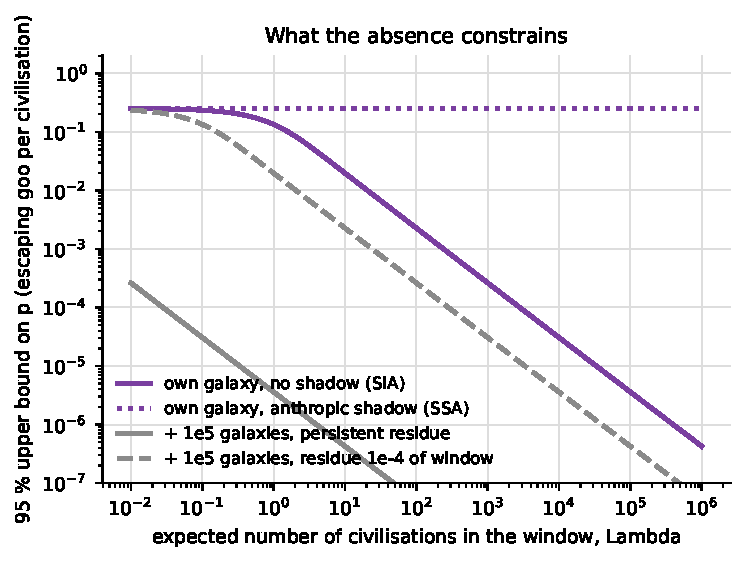
\includegraphics[width=0.75\textwidth]{fig5_bayes}
\caption{Posterior 95\% upper bound on $p$, the probability per civilisation
of a goo that reaches other stars, against the expected number of
civilisations $\Lambda$ in the 5\,Gyr window, for the four readings of the
data.  Under the anthropic shadow our own galaxy's state is uninformative; the
external-galaxy null is not shadowed and is the binding constraint whenever
the goo's signature persists.}
\label{fig:bayes}
\end{figure}

\begin{table}
\centering
\caption{95\% upper bounds on $p$ (prior-free exclusion; the log-uniform
posterior bounds are within a factor of a few and are given in the released
results).  ``ext'' is the $10^{5}$-galaxy null; ``persist'' a goo that keeps
reprocessing, ``dead'' one visible for $10^{-4}$ of the window.}
\label{tab:bayes}
\begin{tabular}{lcccc}
\toprule
$\Lambda$ & own galaxy, naive & own galaxy, shadowed & ext, persist & ext, dead \\
\midrule
1 & \LbOwnLamOne & --- & \LbExtPersistLamOne & \LbExtDeadLamOne \\
100 & \LbOwnLamHundred & --- & \LbExtPersistLamHundred & \LbExtDeadLamHundred \\
$10^{4}$ & \LbOwnLamTenK & --- & \LbExtPersistLamTenK & \LbExtDeadLamTenK \\
\bottomrule
\end{tabular}
\end{table}

\subsection{What it means for us}
\label{sec:us}

The bounds are on $p=p_{\rm goo}p_{\rm esc}$.  To say anything about
$p_{\rm goo}$---the quantity the risk literature elicits and the one a
civilisation can act on---one must divide by $p_{\rm esc}$, and this is where
the physics of Sections~\ref{sec:planet}--\ref{sec:active} bites.  The
astronomical data multiply the likelihood of the \emph{escaping} branch by a
ratio $\ell<1$ and leave the planet-bound branch untouched, so that an
elicited prior $p_{\rm goo}$ becomes
\begin{equation}
p_{\rm goo}' = p_{\rm goo}\,\frac{(1-p_{\rm esc})+p_{\rm esc}\,\ell}
{1-p_{\rm goo}\,p_{\rm esc}\,(1-\ell)}.
\label{eq:branch}
\end{equation}
Figure~\ref{fig:branch} plots the ratio $p'_{\rm goo}/p_{\rm goo}$ for
$p_{\rm goo}=10^{-3}$.  With $\ell=10^{-3}$---the external-galaxy null at
$\Lambda\sim100$ against a prior of $p\sim10^{-3}$---the update is a factor
\BranchRatioTypical if one per cent of goo accidents reach other stars,
\BranchRatioTenth if a tenth do, and \BranchRatioHalf if half do.  For the
elicited priors in the literature---\citet{Sandberg2008} report a median
0.05\% for an extinction-level nanotechnology accident by 2100 and 5\% for
deliberate nanotechnology weapons; \citet{Ord2020} assigns nanotechnology no
separate value, treating it within his residual anthropogenic categories at
1 in 30 and 1 in 50 per century---the relevant $p_{\rm esc}$ is the fraction of
\emph{our} plausible accidents that would be interstellar.  A molecular
replicator loose in a laboratory, a factory or a field is planet-bound
(Section~\ref{sec:planet}); it becomes system-scale only if released in space
or if the civilisation has space industry for it to eat; it becomes
interstellar-passive only if it is both in space and below the blowout size,
and interstellar-active only if it inherits a starship.  For a civilisation at
our stage $p_{\rm esc}$ is small, and equation~(\ref{eq:branch}) says the
astronomical silence changes $p_{\rm goo}$ by a factor within a per cent of
unity.  The contact graph of Section~\ref{sec:contact} closes the one loophole
in that statement: the natural routes off a planet---impact ejecta, grazing
bodies captured elsewhere---deliver $R_{0}\ll1$ strict touches in the field,
so a planet-bound goo stays planet-bound unless it is put among the small
bodies on purpose.

\begin{figure}
\centering
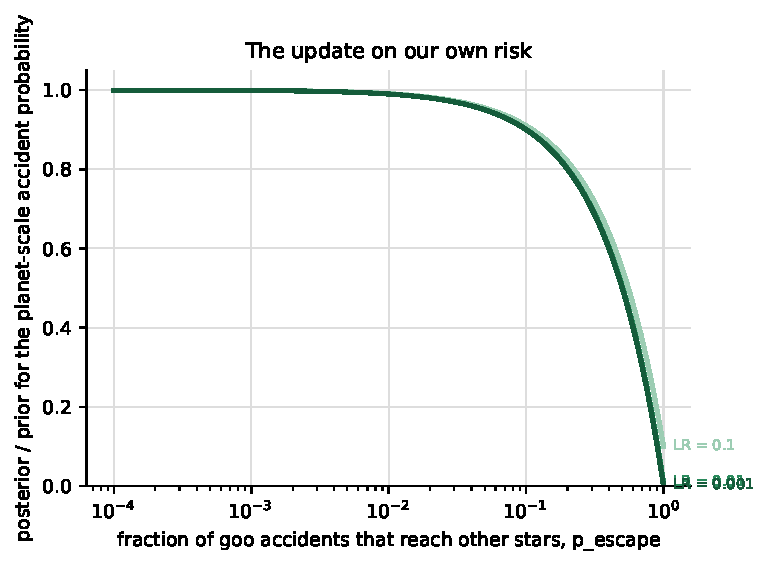
\includegraphics[width=0.7\textwidth]{fig6_branch}
\caption{The update on the planet-scale accident probability $p_{\rm goo}$
implied by an astronomical likelihood ratio $\ell$ on the escaping branch, as
a function of the fraction $p_{\rm esc}$ of accidents that reach other stars.
The planet-bound branch is untouched; only a civilisation whose accidents
would mostly be interstellar learns much from the sky.}
\label{fig:branch}
\end{figure}

This is the paper's central conclusion and we state it plainly.  \emph{The
astronomical record is informative about goo that travels and silent about goo
that stays home, and the goo a civilisation at our stage can accidentally
make is the kind that stays home.}  It should not reassure us about the
planetary risk; it does not raise it either.  What it does say, with force
proportional to $\Lambda$, is that a self-replicating machine population that
keeps growing across a galaxy is not a common end of civilisations---the
external bound is $p<\LbExtPersistLamHundred$ if a hundred civilisations
have arisen per galaxy---and that the classical berserker and
runaway-probe scenarios are constrained by the same data that constrain
Kardashev-III engineering.  For the passive branch the constraint is on the
product of $p$ with the interstellar survival of a machine, and we cannot
separate them.

Two corollaries follow for the Great Filter.  \citet{Hanson1998} and
\citet{Bostrom2008} argue that a filter ahead of us is the pessimistic
reading of the silence, and Bostrom that finding independent life nearby
would be bad news because it moves the filter forward.  Goo is a candidate
late filter, and the present calculation says that if it is one, it is an
\emph{invisible} one: a filter that consumed civilisations on their own planets
would leave a galaxy exactly as quiet as the one we see, and only a filter that
spilled out would have announced itself.  The silence therefore does not
distinguish a planet-bound goo filter from no filter; it distinguishes only
against goo filters that travel.  Conversely, \citet{Cirkovic2004} noted that
catastrophic explanations of the silence have an optimistic side---they are
consistent with life being common---and a planet-bound goo filter has that
property in full.

\section{The other replicators}
\label{sec:general}

The argument does not depend on the replicator being molecular.  It depends
on three things: that the population grows without external limit, that its
reach is set by dispersal, and that its astronomical visibility is set by
whether it keeps metabolising where a survey can see.  Table~\ref{tab:general}
runs the other self-replicating technologies with which a civilisation could
end itself through the same three questions.  Engineered organisms
\citep{Millett2017,Esvelt2022} and mirror life \citep{Adamala2024} are
planet-bound by construction: their dispersal is the biosphere's, their reach
the biosphere's, and their astronomical signature at most the loss of a
biosignature.  Gene drives \citep{Noble2018} are the same with a smaller
substrate.  Macroscopic self-replicating machines---the lunar factory of
\citet{Freitas1980b}, the ``clanking replicators'' of \citet{Moses2020}, the
space-industry bootstraps of \citet{Metzger2013}---are system-scale by
construction and are the branch the waste-heat surveys already bound; their
units are too large for passive escape and their reach stops at the system
unless they inherit a ship.  Computational replicators---network worms
\citep{Moore2003,Staniford2002} and, latterly, self-replicating AI agents
\citep{Pan2024}---have the fastest doubling times of any replicator ever
built (the Slammer worm doubled every 8.5\,s and infected $75\,000$ hosts in
ten minutes) and the smallest reach: the substrate is the network, and the
network stops at the edge of the civilisation's own hardware.  Their
astronomical signature is nil unless they capture the physical economy, at
which point they are one of the other rows.  Only the deliberately
interstellar replicator---the probe---has a reach the sky can see, and it is
the one replicator whose safety a civilisation designs on purpose.

\begin{table}
\centering
\small
\caption{The other self-replicating technologies a civilisation could die of,
by the three properties that govern reach and visibility.}
\label{tab:general}
\begin{tabular}{p{3.0cm}p{2.0cm}p{2.6cm}p{2.6cm}p{3.6cm}}
\toprule
replicator & doubling & dispersal & reach & astronomical signature \\
\midrule
molecular assembler & $10^{2}$--$10^{4}$\,s & none / space / blowout / ship & planet / system / annulus / galaxy & none / waste heat / seeding / front \\
engineered organism, mirror life & hours & biosphere & planet & loss of a biosignature \\
gene drive & generations & population & planet & none \\
macroscopic machine, space industry & months--years & space transport & system & waste heat at the feedstock's orbit \\
network worm, AI agent & seconds--hours & network & the civilisation's hardware & none, unless it takes the economy \\
von Neumann probe & years & starship & galaxy, cosmos & front; Kardashev-III reprocessing \\
\bottomrule
\end{tabular}
\end{table}

The general lesson is the same as the specific one.  Accidental replicators
inherit the dispersal of the environment they escape into, and for a
civilisation at our stage that environment is a planet.  The astronomical
silence is therefore a statement about the one class of replicator we would
have to build on purpose, and about the civilisations that built it.  A
companion paper develops this generalisation and its policy content.

\section{Discussion}
\label{sec:discussion}

\paragraph{Assumptions that matter.}  The calculation assumes substrate
generality: a device that eats an asteroid can eat a planet's surface, and one
intact seed suffices.  Nothing we know of can do this, and
\citet{PhoenixDrexler2004} and \citet{Freitas2000} argue that nothing easily
could; the paper's numbers are conditional on the accident having happened.
It assumes the error catastrophe does not end the goo before the scale in
question is reached.  \citet{Kowald2015} argues that finite-fidelity copying
makes an optimal probe design fail on a bounded number of generations, and the
active branch is the most exposed: $10^{4}$ hops across the Galaxy is $10^{4}$
generations at least.  A goo that dies of copying errors before it crosses the
Galaxy is, for our purposes, a system-scale goo, and the inference moves it
to that row.  It assumes no competition: \citet{Chen2022} show that
predator--prey dynamics between replicator strains can hold a population far
below the feedstock limit.  And the passive branch and the contact graph assume a
functional survival time that no one has measured for anything but grains;
for rock-borne carriers the paper takes survival for granted and lets the
number of carriers decide.

\paragraph{Live versus dead.}  The single most consequential result is
equation~(\ref{eq:tvis}).  It means that a goo that stops is invisible on any
timescale a survey samples, and that what the waste-heat surveys bound is a
goo that never stops.  Whether a real goo would stop---exhausting its
feedstock, losing to its own mutants, or grinding into fragments it can no
longer use---is the question on which the system-scale bound turns, and it is
a question about the design of replicators, not about astronomy.

\paragraph{The anthropic choice.}  We have shown both readings of our own
system's silence.  We note that the choice does not change the conclusion in
Section~\ref{sec:us}, because that conclusion rests on the external galaxies,
which no reading shadows.  It does change what one may say about the passive
branch, whose gigayear timescale means the external galaxies are unaffected by
it (an annulus in another galaxy is no less consumed for being far away) but
whose signature is not a galaxy-wide reprocessing: a passively seeded annulus
is a set of consumed systems, each of which is visible only while alive.  The
passive branch is therefore bounded by the system-scale surveys, not by \Ghat,
and the bound is weaker by the ratio of the survey volume to the Galaxy.

\paragraph{What would change the answer.}  Three observations would.  A
temperate rocky planet with a refined, uniform surface and no atmosphere
chemistry---the planetary residue---is beyond current instruments but not
beyond a large direct-imaging telescope; a single such detection would be the
first entry in the planetary row.  A debris disc around an old, metal-poor or
halo star, where no natural reservoir can make one (this repository's
OSSUARY channel; \citealt{Lacki2025} named the population), would be the
system-scale residue in the one place its natural background is absent.  And
a swarm whose temperature matches its host's belt rather than its habitable
zone---waste heat where the rock was, not where the energy is wanted---would
be the discriminant between goo and purpose in any future Dyson candidate.

\section{Conclusions}
\label{sec:conclusions}

\begin{enumerate}
\item No published work computes the propagation of an uncontrolled
self-replicator beyond its planet, compiles the observational constraints on
it, or draws the implication for the civilisation asking.  This paper does
all three.
\item Replication rate is almost never the bottleneck.  In place, a planet's
crust is a \CrustGovTime project and its bulk a \BulkGovTime one at any
doubling time, because the surface cannot shed the heat faster; a planetary
system's small bodies are transport-limited to \BeltConvTime--\KuiperConvTime;
the Galaxy is a \FillFastFast--\FillSlowSlow project for an active front and
a \AnnulusFillGyr\,Gyr one for a passive cloud.  Dispersal class, decided at
the micron and at the shipyard, sets the reach.
\item A detectable dead residue is a short-lived one: at most
$P_{\rm orb}/f_{\min}$ above the detection floor.  The waste-heat surveys bound
live goo; dead goo is invisible on any timescale surveyed.
\item A replicator smaller than \BlowoutRadiusUm\um leaves its system on
starlight alone, and the \WindowLoUm--\WindowHiUm\um class reaches the next
habitable zone; a single belt-scale release seeds every rocky planet in the
solar annulus within a gigayear if the devices survive $\gtrsim10^{8}$\,yr in
the interstellar medium.  Passive goo has no front; it has a cloud.
\item The contact graph of the Galaxy is already complete in the mass sense:
every Earth-sized planet has been struck tens of times by interstellar
objects, every system is inside every other's planetesimal cloud, and one
system's ejecta are captured by $\sim10^{7}$ others.  For one system's material
\emph{landing} on other planets the graph is at threshold
($R_{0}\approx\IsoRZeroStrict$ by interstellar objects, $10^{-3}$ by impact
ejecta, $10^{19}$ by dust-sized carriers), so contact is never the bottleneck
for a replicator among a system's small bodies and never the route for one
confined to a planet; survival and size are.
\item The observational record constrains, per civilisation,
$p\lesssim\LbExtPersistLamHundred$ for a persistent galaxy-spanning goo at
$\Lambda=100$, from the $10^{5}$-galaxy null, which is neither anthropically
shadowed nor short-memoried; our own system's silence constrains nothing under
the shadow and $p\lesssim\LbOwnLamHundred$ without it.
\item Mapped onto the planet-scale accident probability that a civilisation at
our stage can act on, the silence changes it by a factor \BranchRatioTypical
if one per cent of accidents would be interstellar.  The sky is informative
about goo that travels and silent about goo that stays home; ours would stay
home.
\end{enumerate}

\section*{Data and code availability}
The model, configuration, tests and figure code are in the \texttt{seti.goo}
package of the accompanying repository; \texttt{python -m seti.goo.run --stage
all} regenerates every number in this paper from \texttt{config/goo.yaml}.  The
compiled observational record cites public surveys; the in-house channel
results referenced in Table~\ref{tab:record} are committed under
\texttt{results/} in the same repository.

\section*{Acknowledgements}
[To be added.]

\bibliography{refs}
\end{document}
